\documentclass[fontset=windows]{article}
\usepackage[margin=1in]{geometry}%设置边距,符合Word设定
\usepackage[UTF8]{ctex}
\usepackage{setspace}
\usepackage{amsmath}
\numberwithin{figure}{section}
\usepackage{array}
\usepackage{lipsum}
\usepackage{float}
\usepackage{graphicx}%插入图片
\usepackage[dvipsnames]{xcolor}
\usepackage{authblk}
\usepackage{listings,matlab-prettifier}
\lstset{
	language=Matlab, % 设置代码语言为Matlab
    basicstyle=\ttfamily, % 设置字体为等宽字体
    numbers=left, % 行号在左边显示
    numberstyle=\tiny, % 设置行号字体大小
    stepnumber=1, % 行号递增步长
    numbersep=5pt, % 行号到代码的距离
    backgroundcolor=\color{gray!10}, % 设置代码的背景颜色
    showspaces=false,
    showstringspaces=false,
    showtabs=false,
    frame=single, % 设置代码框
    rulecolor=\color{black},
    tabsize=2,
    breaklines=true,
    breakatwhitespace=true,
    title=\lstname,
	keywordstyle=\bfseries\color{NavyBlue},
	morekeywords={var,};
	emphstyle=\bfseries\color{Rhodamine}, % 强调词样式设置
    commentstyle=\itshape\color{black!50!white}, % 设置注释样式,斜体,浅灰色
    stringstyle=\bfseries\color{PineGreen!90!black}, % 设置字符串样式
	columns=flexible,
}
\graphicspath{{Figures2/}}%文章所用图片在当前目录下的 Figures目录

\usepackage{hyperref} % 对目录生成链接,注:该宏包可能与其他宏包冲突,故放在所有引用的宏包之后
\hypersetup{colorlinks = true,  % 将链接文字带颜色
	linkcolor=black, % 将链接文字黑色
	bookmarksopen = true, % 展开书签
	bookmarksnumbered = true, % 书签带章节编号
	} % 作者
\bibliographystyle{plain}% 参考文献引用格式

\renewcommand{\contentsname}{\centerline{目录}} %经过设置word格式后,将目录标题居中

\title{\heiti\zihao{2} 《统计信号处理》第二教学单元研讨题}
\author{杨 鼎,韦可雷,高司博,高涵博}
\date{}

\begin{document}
\maketitle
\thispagestyle{empty}

%\begin{abstract}
%	\lipsum[2]
%\end{abstract}

%\tableofcontents
%\setcounter{page}{0}
%\newpage

\section{第一题}
什么叫做完备的充分统计量?如何利用完备的充分统计量估计未知参数?由充分统计量是否能够获得MVUE?
获得最大似然估计的途径有哪些?最大似然估计与有效估计量、充分统计量、MVUE之间是否有联系?
可举例验证你的观点。

\subsection*{(1)什么叫做完备的充分统计量?}

1.充分性条件:如果\(PDFp(\mathbf{x};\theta)\)能够分解为
\begin{align*}
	p(\mathbf{x};\theta)=g(T(\mathbf{x},\theta))h(\mathbf{x})
\end{align*}
其中g为只是通过\(T(\mathbf{x})\)才与\(\mathbf{x}\)有关的函数,
h只是\(\mathbf{x}\)的函数,那么\(T(\mathbf{x})\)是\(\theta\)的充分统计量。

2.完备性条件:如果对所有的\(\theta\),条件
\begin{align*}
	\int_{-\infty}^{\infty} v(T)p(T;\theta)dT=0
\end{align*}
只对零函数\(v(T)=0\)(对所有的T)满足,那么,我们就说充分统计量是完备的。

\subsection*{(2)如何利用完备的充分统计量估计未知参数?}

利用RBLS定理

如果\(\check{\theta}\)是\(\theta\)的无偏估计量,\(T(x)\)是\(\theta\)的充分统计量,
那么\(\check{\theta}=E(\check{\theta|T(x)})\)是

1.\(\theta\)是一个适用的估计量(与\(\theta\)无关);

2.无偏的;

3.对所有的\(\theta\),它的方差要小于或等于\(\check{\theta}\)的方差;

4.特别地,当\(T(x)\)是完备的充分统计量时,\(\check{\theta}\)是MVU估计量。

\subsection*{(3)由充分统计量是否能够获得MVUE?}
根据BRLS定理,如果充分统计量\(T(\mathbf{x})\)是完备的,那么它就是MVUE。
1.利用Neyman-Fisher因子分解定理来求一个\(\theta\)的统计量,即\(T(\mathbf{x})\);

2.确定充分统计量是否完备,如果是,继续往下进行;否则这个方法不能使用;
3.求一个充分统计量的函数,以此来得到一个无偏估计量\(\hat{\theta}=g(T(\mathbf{x}))\),
那么\(\hat{\theta}\)就是MVUE。或者,计算\(\hat{\theta}=E(\check{\theta}|T(\mathbf{\theta}))\)
,其中\(\check{\theta}\)是任意无偏估计量。

\subsection*{(4)获得最大似然估计的途径有哪些?}
1.写出似然函数,求出使得似然函数最大的估计量\(\hat{\theta}\)

2.已知充分统计量\(T(\mathbf{x})\),根据Neyman-Fisher因子分解定理,
极大似然函数最大化等价于\(g(T(\mathbf{x},\theta))\)的最大化,
因此求得使\(g(T(\mathbf{x},\theta))\)关于\(\theta\)最大化的估计量即为MLE。

\subsection*{(5)最大似然估计与有效估计量、充分统计量、MVUE之间是否有联系?}
有效估计量:无偏且达到CRLB的估计量。

充分统计量:包含待估计量所有信息的统计量。

MVUE:在无偏估计的前提下,使得方差最小的估计量。

MVUE估计量和有效估计量都是无偏的,但MVUE不一定是有效估计量(见教材图3.2);
根据教材定理7.1,最大似然估计量可以视为渐进无偏的和渐进达到CRLB,因此它是渐进有效的;
根据Neyman-Fisher因子分解定理,对于充分统计量\(T(\mathbf{x})\),PDF可以分解为
\(p(T(\mathbf{x});\theta)=g(T(\mathbf{x},\theta))h(\mathbf{x})\),
求MLE时,使似然函数最大化,等价于使\(g(T(\mathbf{x},\theta))\)关于\(\theta\)求得极大值,
因此,MLE是充分统计量\(T(\mathbf{x})\)的函数。

\section{第二题}
考虑高斯噪声中正弦信号参数估计问题。观测模型为
\begin{align*}
	x_n=A\cos2\pi f_0 n+w_n,n=0,1,…,N-1
\end{align*}
其中\(w_n\)为零均值高斯噪声。

\subsection*{(1)当\(w_n\overset{i.i.d}{\sim} N(0,\sigma^2)\),\(f_0\)、\(\sigma^2\)均已知,
	你认为可以用哪些方法对参数A进行估计?}

\subsection*{(2)\(A=1,\sigma^2=0.1\)时,绘制频率参数的克拉美-罗下限曲线,
	并解释你观察到的现象。}

\subsection*{(3)\(A=1,f_0=0.25,f_0=0.05\)时,分别对频率参数的最大似然估计进行仿真,绘制参数估计性能随样本量、信噪比的变化曲线,
	并与克拉美-罗下限进行对比;分析验证最大似然估计的渐进性能。}

当\(A=1\)时,极大似然函数为
\begin{align*}
	p(\mathbf{x};f_0)=\frac{1}{(2\pi \sigma^2)^{\frac{N}{2}}}
	\exp\left\{-\frac{1}{2\sigma^2}\sum_{n=0}^{N-1}\left[x[n]-\cos2\pi f_0n\right]^2\right\}
\end{align*}
使得似然函数最大,等价于使指数项
\begin{align*}
	J(f_0)=\sum_{n=0}^{N-1}\left[x[n]-\cos2\pi f_0n\right]^2
\end{align*}
最小。对于集合\((0,1/2)\)内的所有\(f_0\),利用网格搜索法,可以求出\(J(f_0)\)的最小值,这时的\(f_0\)即为MLE。

\newpage

\subsection*{(4)如果\(w_n\)为零均值高斯色噪声,可用如下AR模型描述
	\begin{align*}
		w_n=aw_{n-1}+e_n
	\end{align*}
	其中,\(e_n\overset{i.i.d}{\sim}N(0,\sigma_e^2),a=0.8,A=1\),试问什么情况下能够获得更准确的频率参数估计?
	试与白噪声的情况进行比较(相同的噪声方差下)。}

重写为矢量形式
\begin{align*}
	\mathbf{x} & =\mathbf{F}+\mathbf{w}           \\
	\mathbf{w} & =\mathbf{H}\mathbf{w}+\mathbf{e}
\end{align*}
其中
\begin{align*}
	\mathbf{x} & =
	\begin{bmatrix}
		x_0 & x_1 & x_2 & \dots & x_n
	\end{bmatrix}^T  \\
	\mathbf{F} & =
	\begin{bmatrix}
		1 & \cos2\pi f_0 & \cos2\pi f_0*2 & \dots & \cos2\pi f_0 n
	\end{bmatrix}^T  \\
	\mathbf{w} & =
	\begin{bmatrix}
		w_0 & w_1 & \dots & w_n
	\end{bmatrix}^T \\
	\mathbf{H} & =
	\begin{bmatrix}
		0      & 0      & 0      & \dots  & 0      & 0      \\
		a      & 0      & 0      & \dots  & 0      & 0      \\
		0      & a      & 0      & \dots  & 0      & 0      \\
		\vdots & \vdots & \vdots & \ddots & \vdots & \vdots \\
		0      & 0      & 0      & \dots  & 0      & 0      \\
		0      & 0      & 0      & \dots  & a      & 0
	\end{bmatrix}   \\
	\mathbf{e} & =
	\begin{bmatrix}
		e_1 & e_2 & \dots & e_n
	\end{bmatrix}^T
\end{align*}
由于\(e_n\overset{i.i.d}{\sim} \mathcal{N} (0,\sigma_e^2),
\mathbf{e}\sim \mathcal{N}(\mathbf{0},\sigma_e^2\mathbf{I})\)。

由\(\mathbf{w}=\mathbf{H}\mathbf{w}+\mathbf{e}\),得到
\((\mathbf{I}-\mathbf{H})\mathbf{w}=\mathbf{e}\),显然\(\mathbf{I}-\mathbf{H}\)可逆,
所以\(\mathbf{w}=(\mathbf{I}-\mathbf{H})^{-1}\mathbf{e}\),
\(\mathbf{x}=A\mathbf{F}+(\mathbf{I}-\mathbf{H})^{-1}\mathbf{e}\)。

已知\(\mathbf{e}=(\mathbf{I}-\mathbf{H})(\mathbf{x}-\mathbf{F})
\sim \mathcal{N}(\mathbf{0},\sigma_e^2\mathbf{I})\)
,所以PDF\(p(\mathbf{x};f_0)\)为
\begin{align*}
	p(\mathbf{x};f_0) & =\frac{1}{(2\pi \sigma_e^2)^{\frac{N}{2}}}
	\exp\left\{ -\frac{1}{2\sigma_e^2}(\mathbf{x}-\mathbf{F})^T(\mathbf{I}-\mathbf{H})^T
	(\mathbf{I}-\mathbf{H})(\mathbf{x}-A\mathbf{F})\right\}        \\
	                  & =\frac{1}{(2\pi \sigma_e^2)^{\frac{N}{2}}}
	\exp\left\{ -\frac{1}{2\sigma_e^2}(\mathbf{x}-\mathbf{F})^T\mathbf{W}
	(\mathbf{x}-\mathbf{F})\right\}
\end{align*}
其中\(\mathbf{W}=(\mathbf{I}-\mathbf{H})^T(\mathbf{I}-\mathbf{H})\),
显然\(\mathbf{W}^T=\mathbf{W}\)。

利用最大似然估计,使似然函数最大,等价于使指数项
\begin{align*}
	J(f_0)=(\mathbf{x}-\mathbf{F})^T\mathbf{W}(\mathbf{x}-\mathbf{F})
\end{align*}
最小。对于集合\((0,1/2)\)内的所有\(f_0\),利用网格搜索法,可以求出\(J(f_0)\)的最小值,
这时的\(f_0\)即为MLE。

\begin{figure}[H]
	\centering
	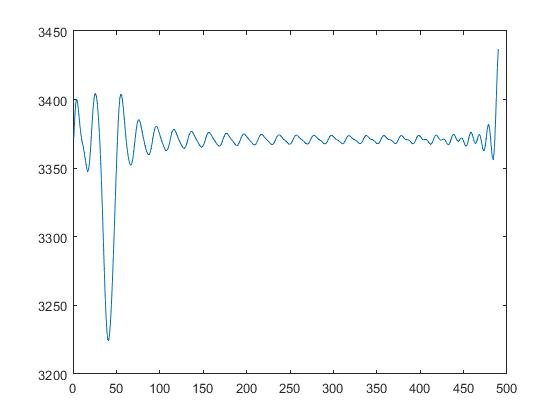
\includegraphics[scale=0.6]{untitled2-2.jpg}
	\caption{通过J的最小值寻找\(f_0\)的MLE原理图}
	\label{2.1}
\end{figure}

图2.1显示了通过网格搜索法求MLE的过程,\(J(f_0)\)对应\(f_0\)值即为MLE。

\begin{figure}[H]
	\centering
	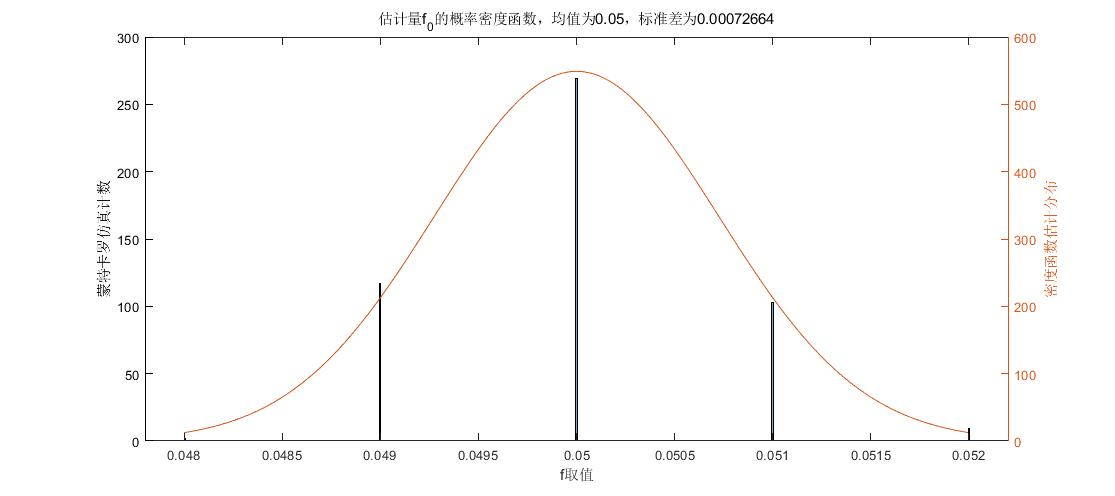
\includegraphics[scale=0.4]{untitled2-1.jpg}
	\caption{蒙特卡洛仿真求得\(f_0\)的MLE的分布图}
	\label{2.2}
\end{figure}

图2.2显示了N=50时,利用蒙特卡洛仿真100次,求得\(f_0\)的MLE的分布直方图与拟合曲线。
图中\(f_0\)分离的取值是由利用网格搜索算法时\(f_0\)的步进长度决定的。
从图中可以看出,蒙特卡洛仿真结果近似服从正态分布,这与最大似然估计的渐渐特性相符。

\begin{figure}[H]
	\centering
	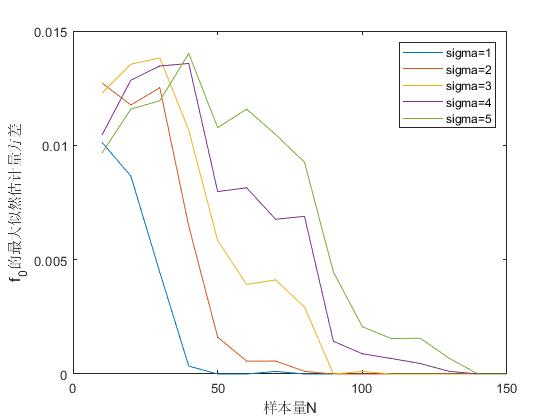
\includegraphics[scale=0.7]{untitled2-3.jpg}
	\caption{不同噪声\(\sigma\)下,\(f_0\)的MLE的方差随样本长度N变化图}
	\label{2.3}
\end{figure}

图2.3显示了不同噪声标准差\(\sigma\)下,随着样本量增加,\(f_0\)的MLE的方差变化曲线。
随着样本长度增加,方差逐渐变小,MLE逐渐趋向于真值。信噪比越低,对应噪声标准差\(\sigma\)越大,
MLE的收敛速度越慢。

\bibliography{books}
\end{document}